\documentclass[aspectratio=169]{beamer}
\setbeamertemplate{navigation symbols}{}
\usepackage{color,amsmath,comment, subfigure}
\usepackage{booktabs}
\usepackage{url}

%%%%%%%%%%%%%%%%%%%%%%%%%%
\title[]{Introduction}
\author[]{Matthew J. Salganik}
\institute[]{Social Network (Soc 204)\\Spring 2021\\Princeton University}
\date[]{Week 1, Lecture 1\\1/2: Scientific overview

\vfill

\begin{flushleft}
\vspace{0.7in}

\includegraphics[width=0.05\textwidth]{figures/cc.png}
\end{flushleft}
}

\begin{document}
%%%%%%%%%%%%%%%%%%%%%%%%%%%
\frame{\titlepage}
%%%%%%%%%%%%%%%%%%%%%%%%%%%
\begin{frame}

\begin{center}
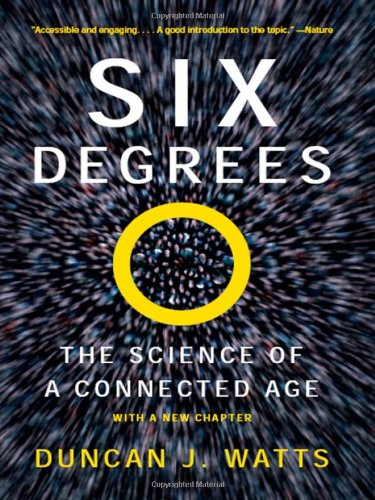
\includegraphics[height=0.50\textheight]{figures/watts_six_2003_cover}
\end{center}

\vfill

\begin{center}
\Large{
We live in the connected age.
}
\end{center}

\end{frame}
%%%%%%%%%%%%%%%%%%%%%%%%%%%
\begin{frame}

\begin{center}
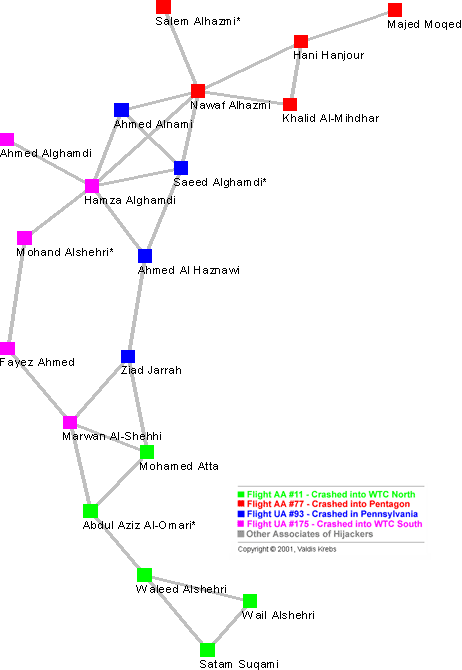
\includegraphics[height=0.90\textheight]{figures/krebs_uncloaking_2002_fig2}
\end{center}

\vfill
\Tiny{\url{http://pear.accc.uic.edu/ojs/index.php/fm/article/view/941/863}}

\end{frame}
%%%%%%%%%%%%%%%%%%%%%%%%%%%
\begin{frame}

\begin{center}
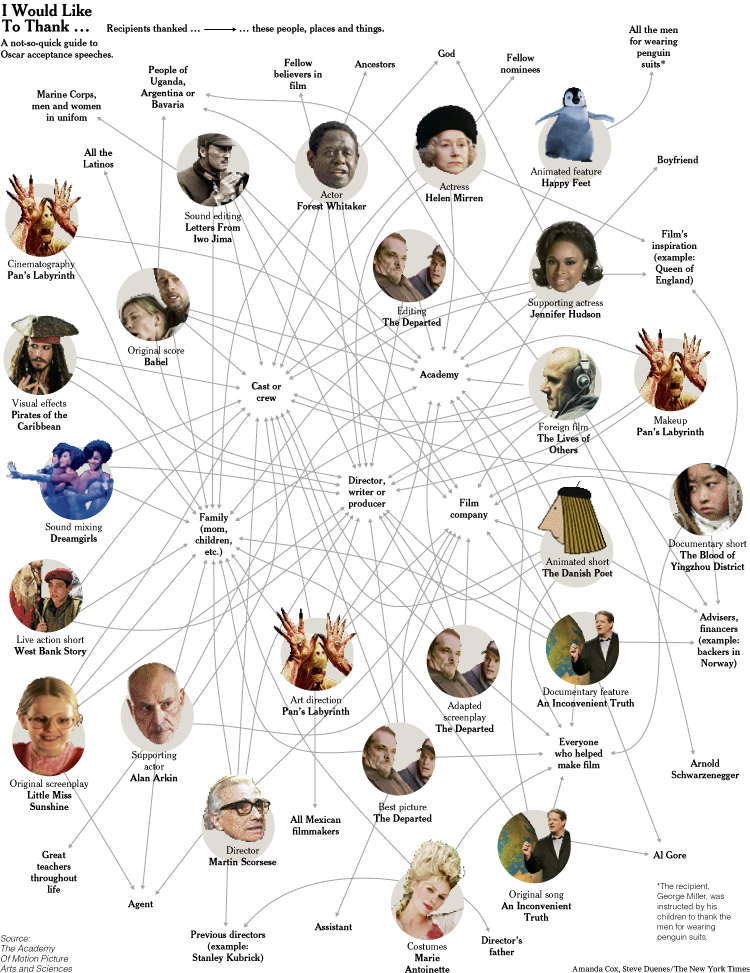
\includegraphics[height=0.9\textheight]{figures/nytimes_oscar_2007}
\end{center}

\vfill
\Tiny{\url{http://www.nytimes.com/imagepages/2007/02/26/movies/27graphic.ready.html}}

\end{frame}
%%%%%%%%%%%%%%%%%%%%%%%%%%%
\begin{frame}

\begin{center}
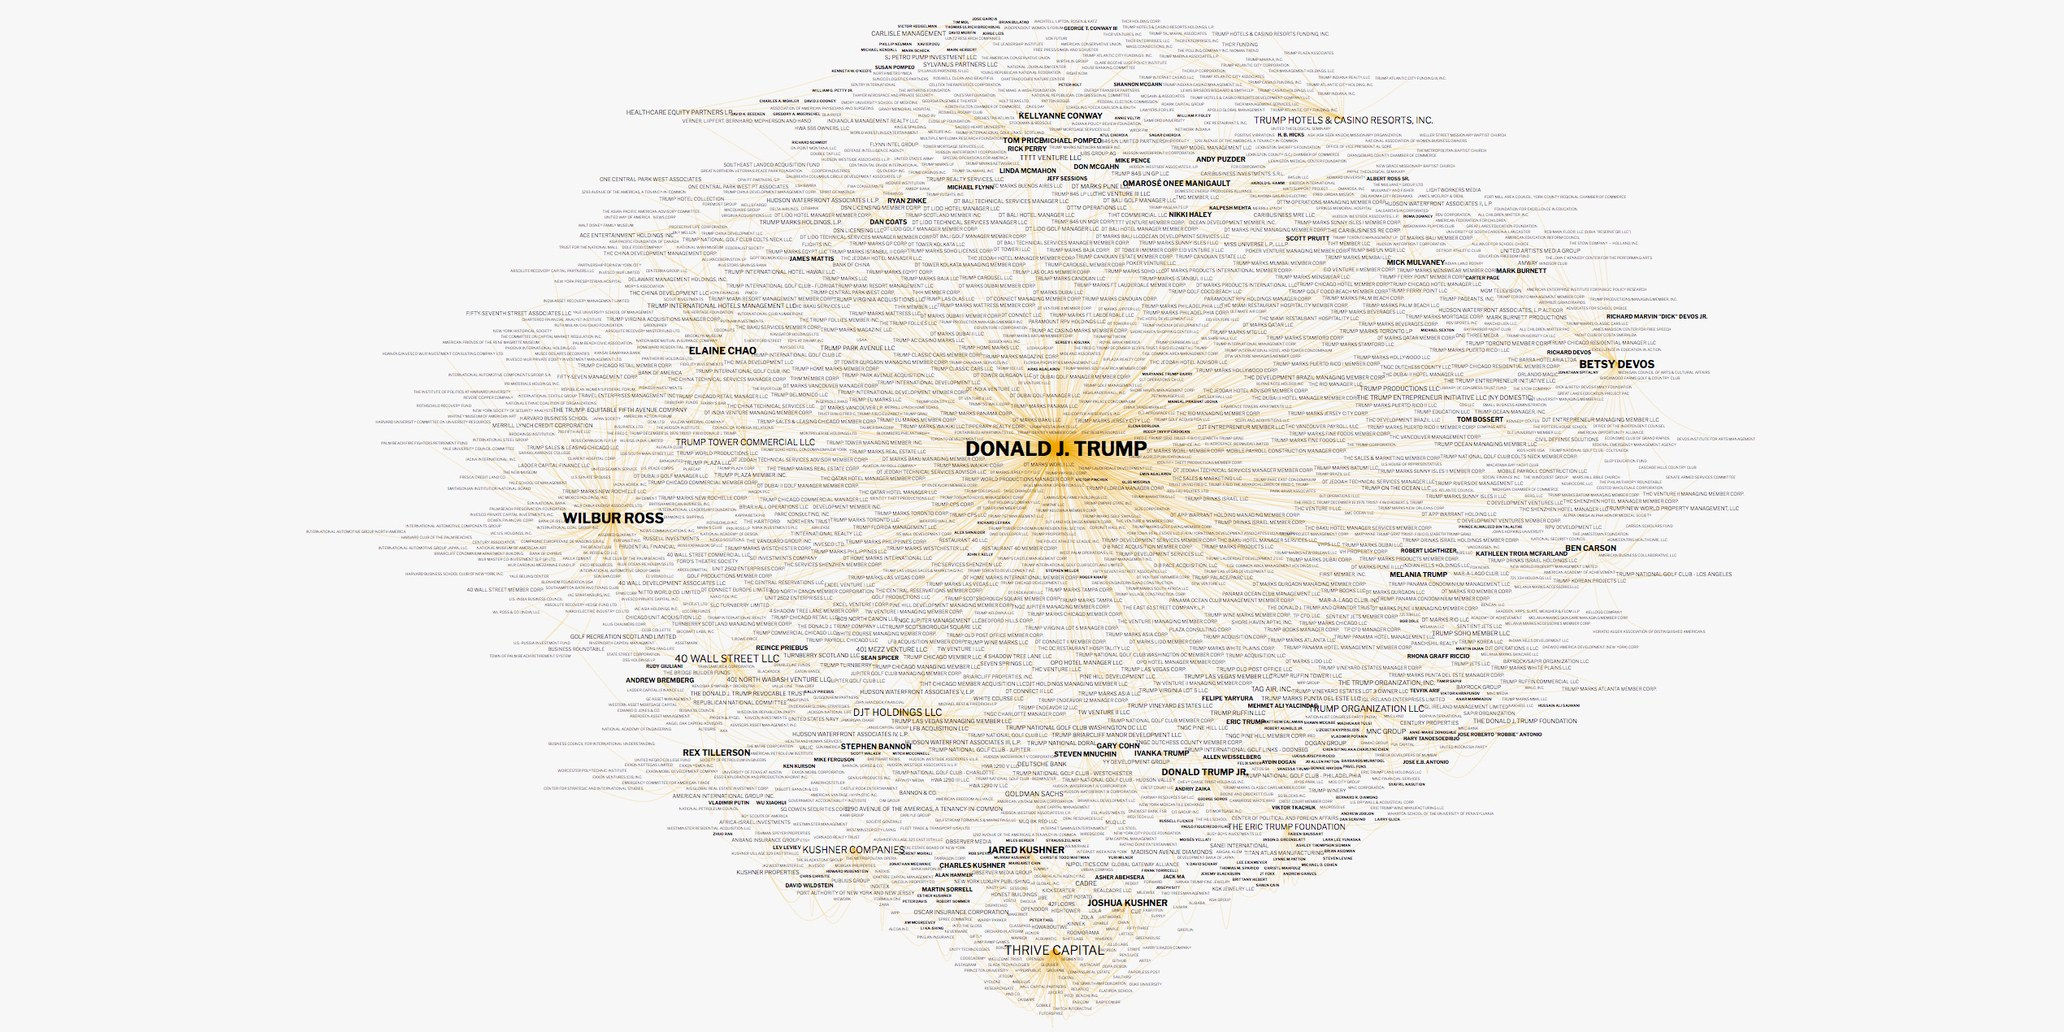
\includegraphics[width=0.9\textwidth]{figures/trump_network}
\end{center}

\vfill
\Tiny{\url{https://kimalbrecht.com/vis/\#trump-connections}}

\end{frame}
%%%%%%%%%%%%%%%%%%%%%%%%%%%
\begin{frame}

General pattern:
\begin{itemize}
\item nodes
\item edges
\end{itemize}

\end{frame}
%%%%%%%%%%%%%%%%%%%%%%%%%%%
\begin{frame}

\begin{center}
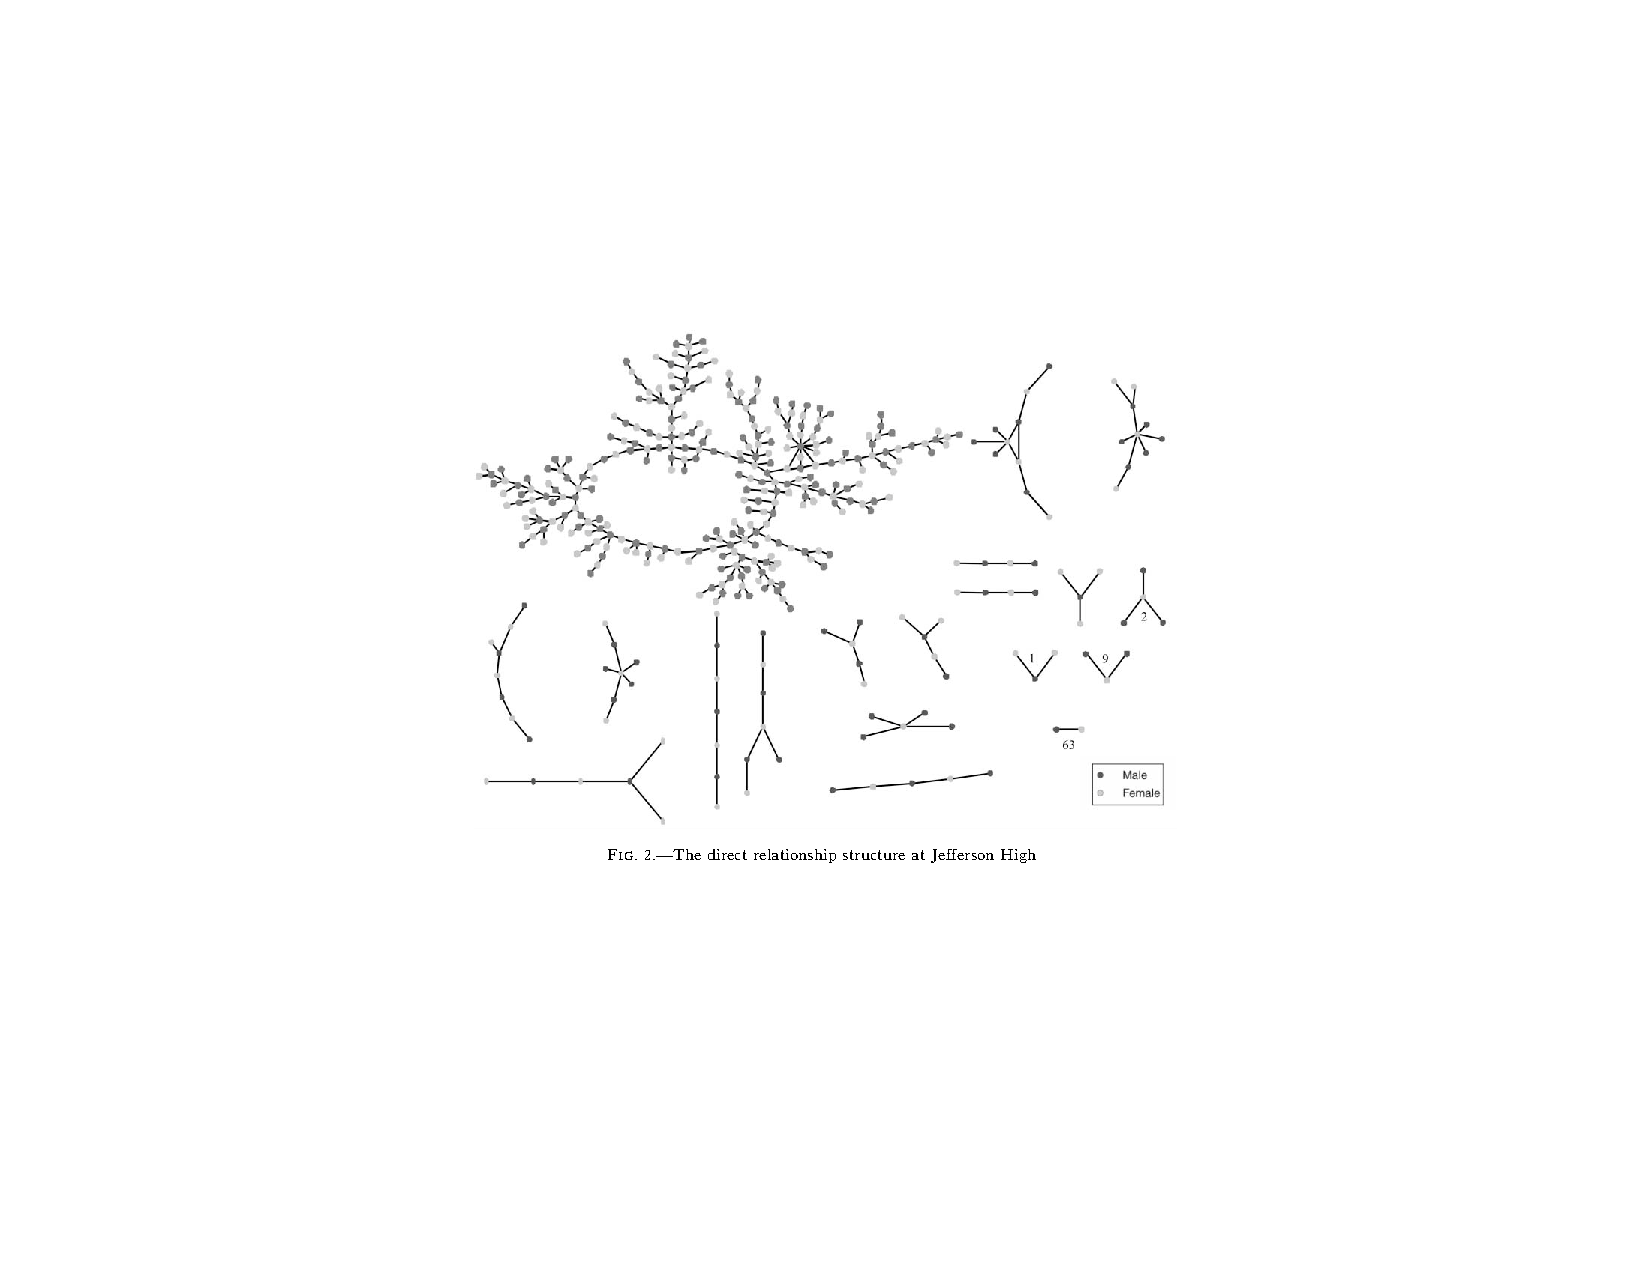
\includegraphics[width=0.95\textheight]{figures/bearman_chains_2004_fig2}
\end{center}

\vfill
\Tiny{url{http://www.journals.uchicago.edu/doi/10.1086/386272}}

\end{frame}
%%%%%%%%%%%%%%%%%%%%%%%%%%%
\begin{frame}
\frametitle{}

\setcounter{subfigure}{0}
\begin{figure}
  \centering
     \subfigure[American High School]{
     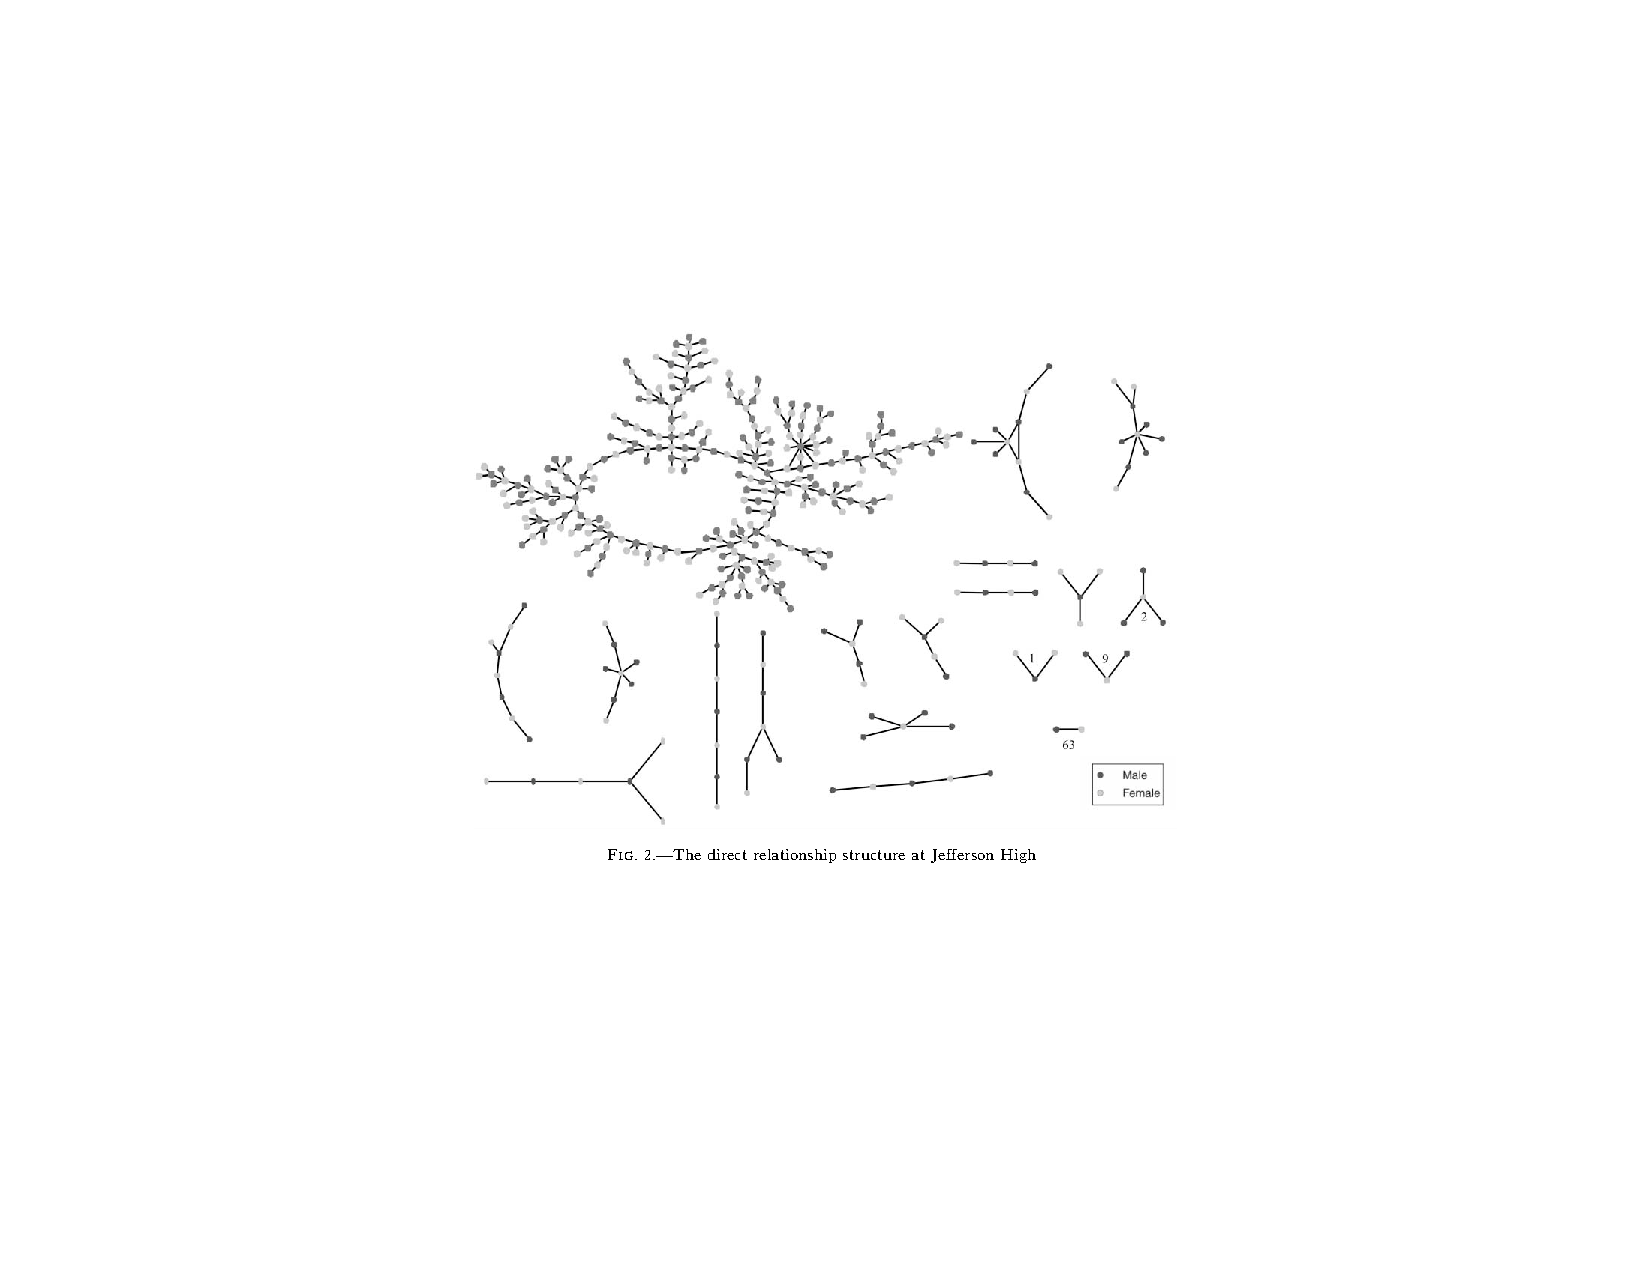
\includegraphics[width=0.45\textwidth]{figures/bearman_chains_2004_fig2}}
  \hspace{0in}
    \subfigure[Likoma Island, Malawi]{
    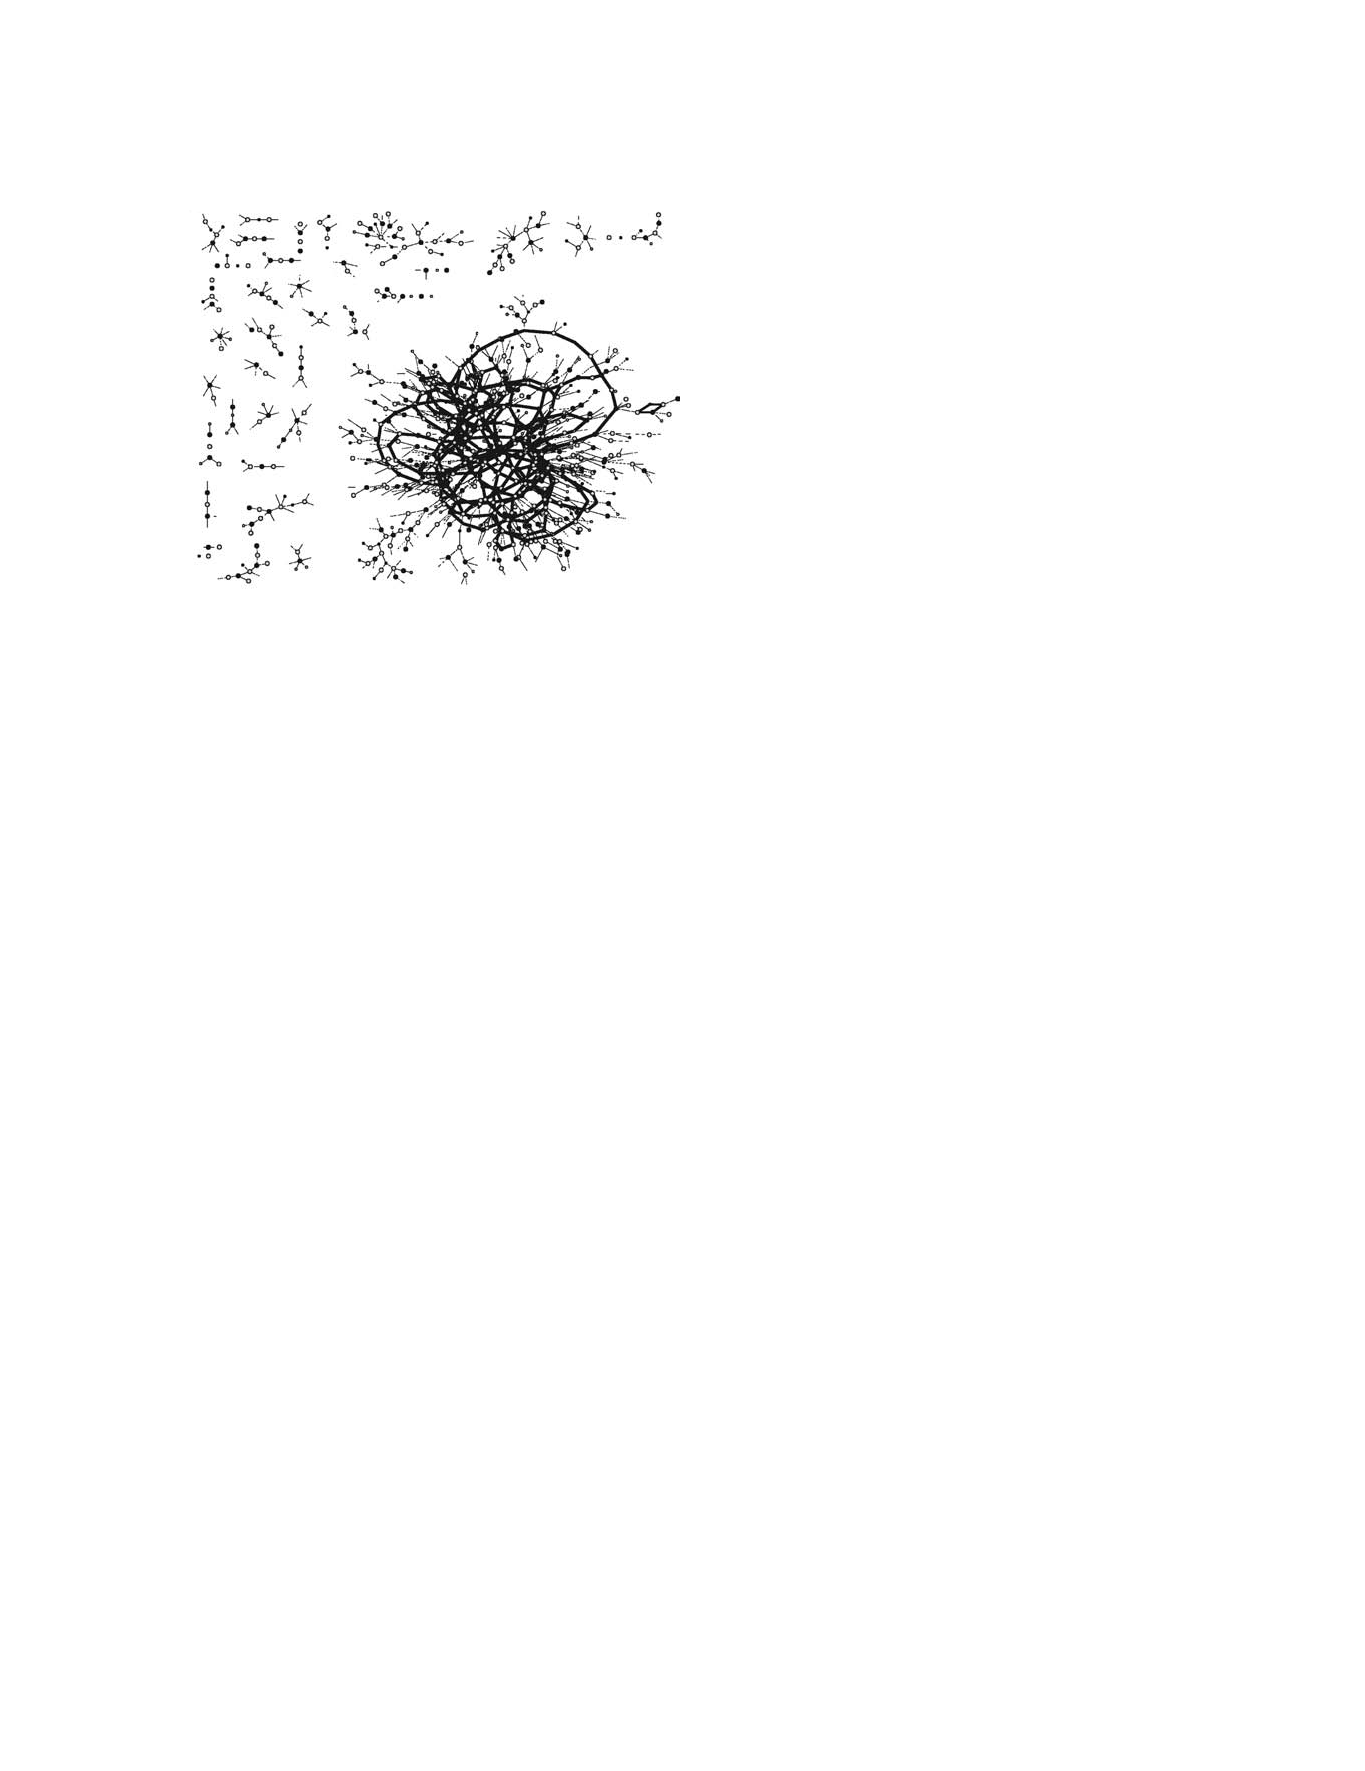
\includegraphics[width=0.45\textwidth]{figures/helleringer_sexual_2007_fig2a}}
\end{figure}

\vfill
\Tiny{\url{http://www.journals.uchicago.edu/doi/10.1086/386272} \& \url{https://www.ncbi.nlm.nih.gov/pubmed/18090281}}

\end{frame}
%%%%%%%%%%%%%%%%%%%%%%%%%%%
\begin{frame}

\begin{center}
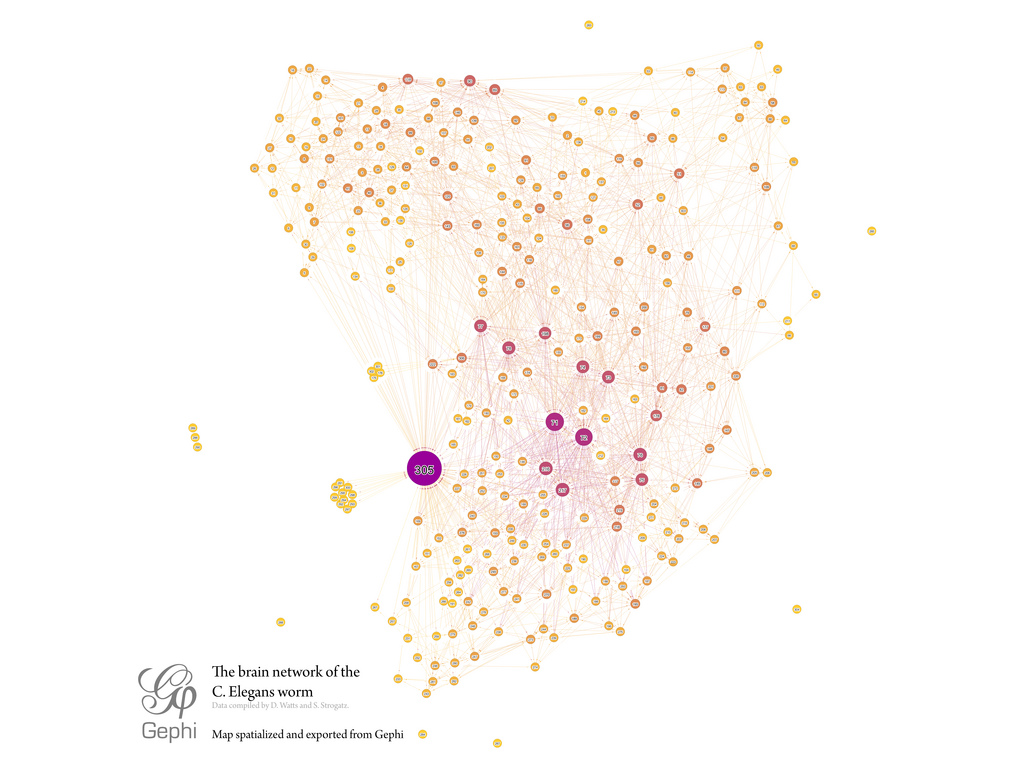
\includegraphics[height=0.9\textheight]{figures/celegans_brain_network}
\end{center}

\vfill
\Tiny{\url{https://commons.wikimedia.org/wiki/File:C.elegans-brain-network.jpg}}

\end{frame}
%%%%%%%%%%%%%%%%%%%%%%%
\begin{frame}
\frametitle{}

\setcounter{subfigure}{0}
\begin{figure}
  \centering
     \subfigure[Worm Brain]{
     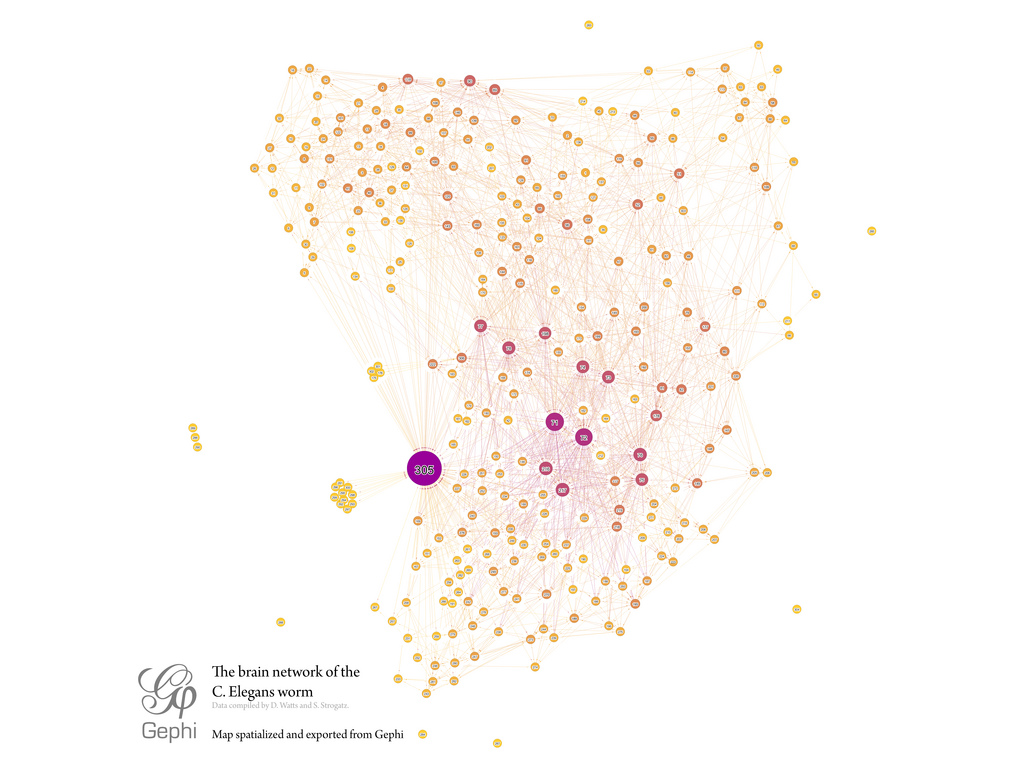
\includegraphics[width=0.45\textwidth]{figures/celegans_brain_network}}
  \hspace{0in}
    \subfigure[Power Grid]{
    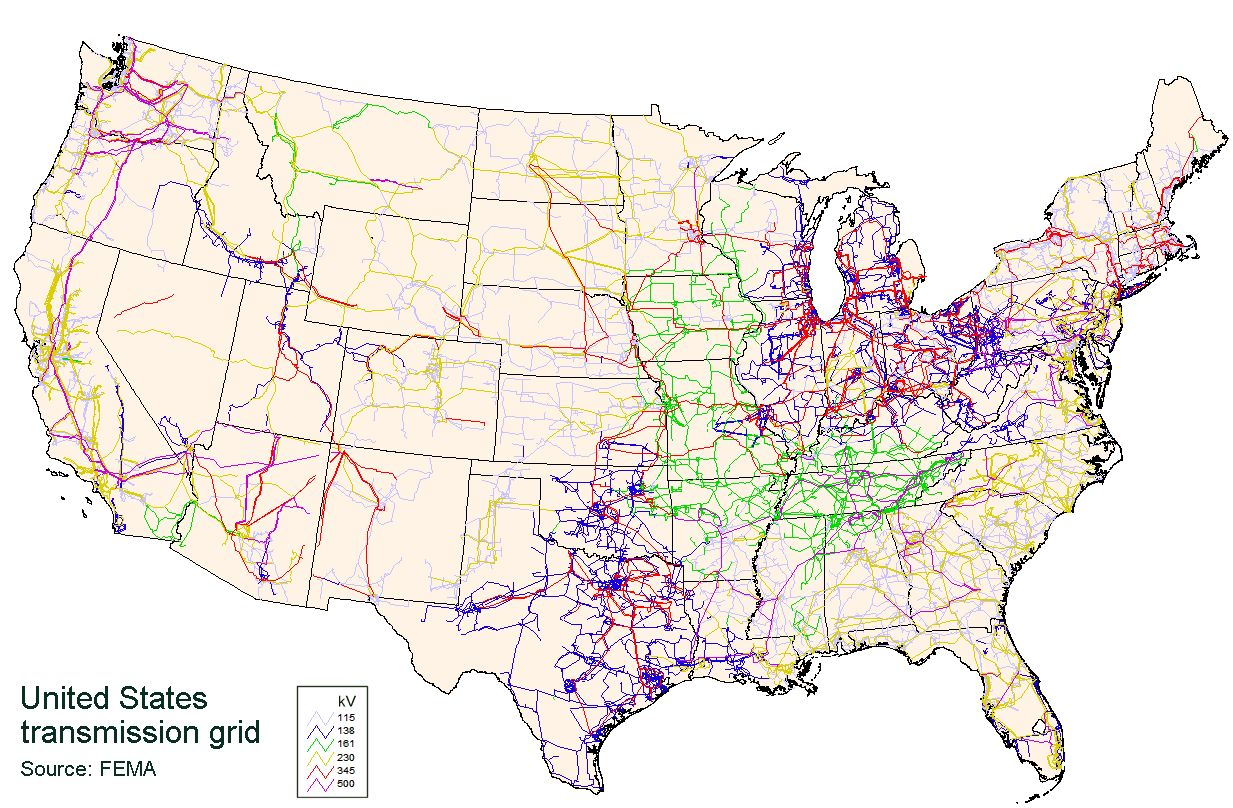
\includegraphics[width=0.45\textwidth]{figures/power_grid}}
\end{figure}

\vfill
\Tiny{\url{https://commons.wikimedia.org/wiki/File:C.elegans-brain-network.jpg} \& \url{https://commons.wikimedia.org/wiki/File:UnitedStatesPowerGrid.jpg}}

\note{
These two have similar structure
We will look not just a social networks but all kinds of networks
}

\end{frame}
%%%%%%%%%%%%%%%%%%%%%%%%%%%
\begin{frame}

\begin{center}
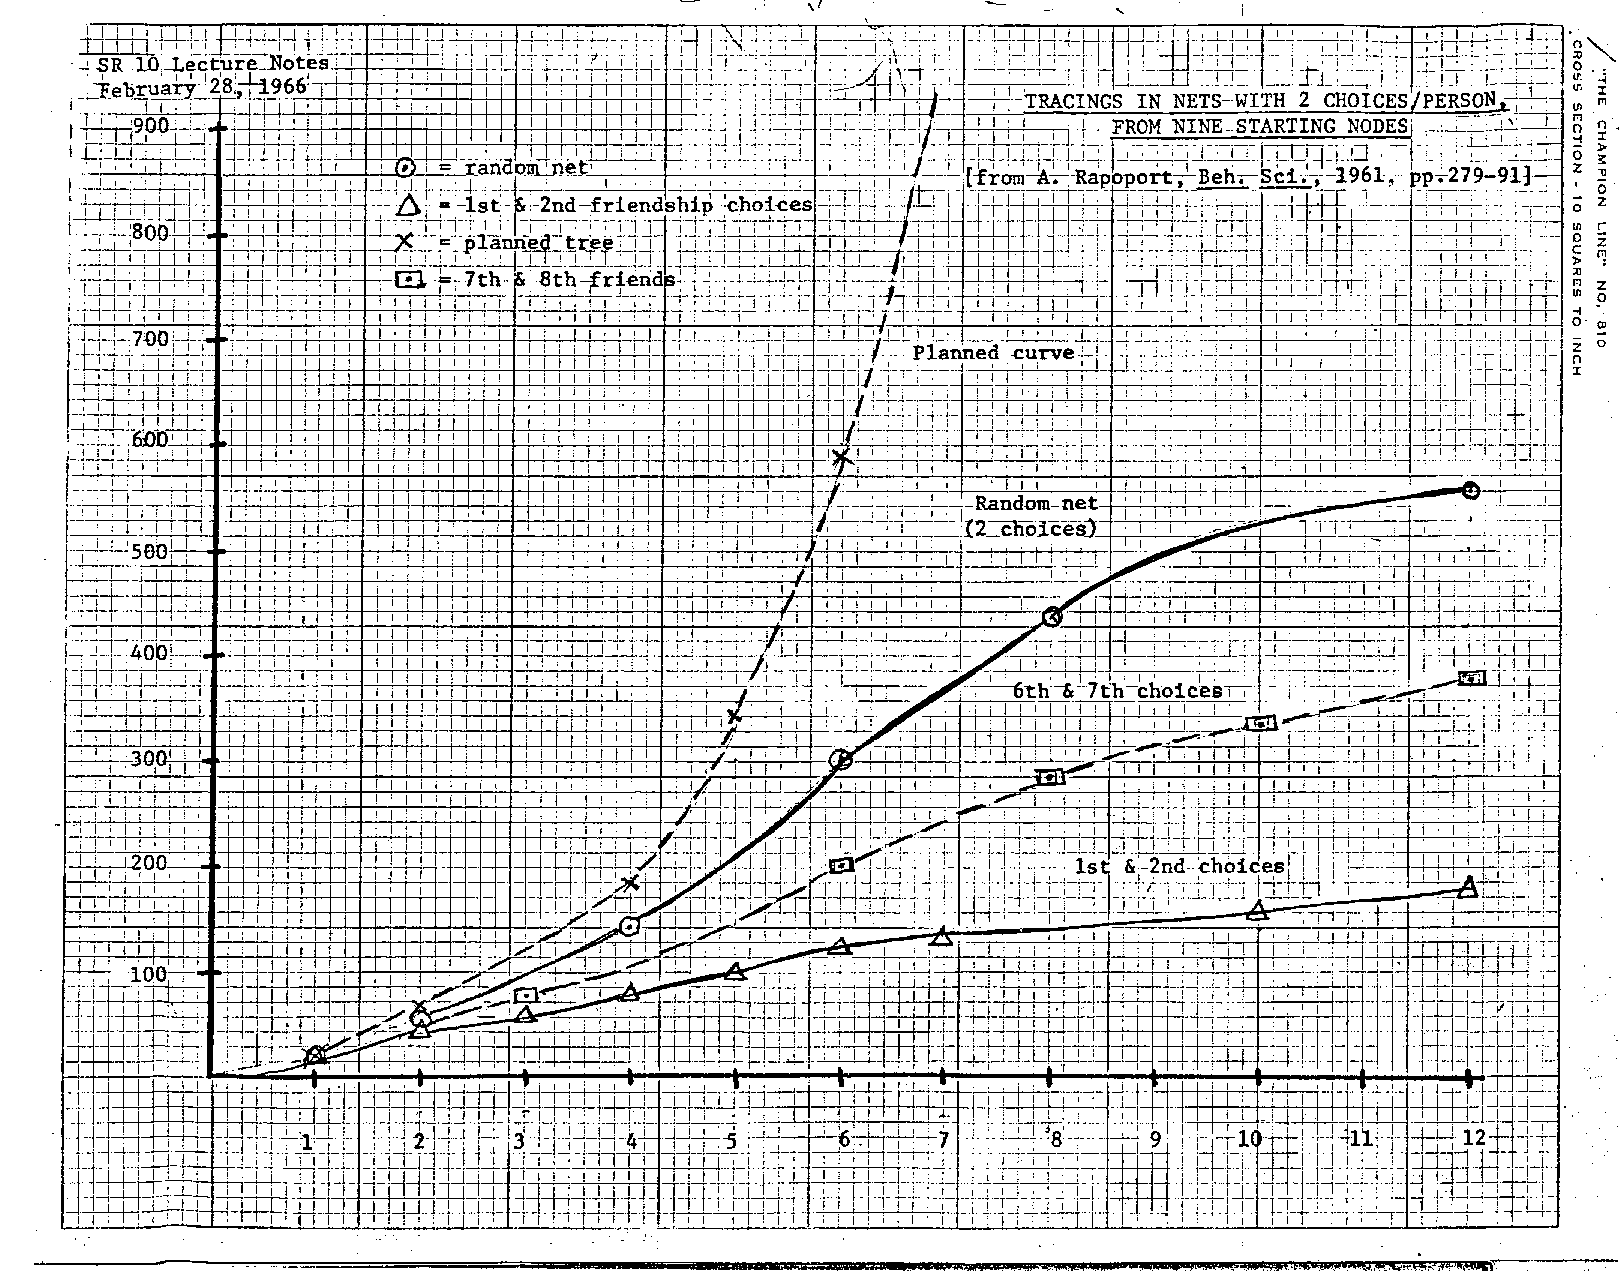
\includegraphics[height=0.9\textheight]{figures/white_classnotes_swt}
\end{center}

\note{
This is not a network in the same way as the others, but it summarizes data from a study from the 50s in middle school in Michigan
This is a graph is from a class taught at Harvard in 1966
This graph explains why you are more likely to get jobs from an acquaintances than close friends
Strength of weak ties
}

\end{frame}
%%%%%%%%%%%%%%%%%%%%%%%%%%%
\begin{frame}

\begin{center}
\Large{Learning objectives}
\end{center}

\end{frame}
%%%%%%%%%%%%%%%%%%%%%%%%%%%
\begin{frame}

\begin{itemize}
\item Students will be able to \textbf{describe} the major concepts used in the study of networks.
\pause
\item Students will be able to \textbf{describe} the interconnections between the major concepts used in the study of networks.
\pause
\item Students will be able to \textbf{use} the major concepts in the study of networks to gain insight into real-world phenomena.
\pause
\item Students will be able to \textbf{evaluate} real, modern research that connects the concepts of networks to real-world phenomena.
\end{itemize}

\note{
Next video we will talk more concretely about what will happen in class
}

\end{frame}
%%%%%%%%%%%%%%%%%%%%%%%%%%%


\end{document}
